\documentclass[usenatbib]{tjaa}

\usepackage[utf8]{inputenc}
\usepackage{lipsum}
\usepackage{cite}
\usepackage{amsmath,amssymb,amsfonts}
\usepackage{algorithmic}
\usepackage{graphicx}
\usepackage{textcomp}
\usepackage{xcolor}
\usepackage{wrapfig}
\usepackage{subcaption}
\usepackage{subfig}
\usepackage{pdfpages}
\usepackage[font=small,labelfont=bf]{caption} % If you are using the caption package
\newsavebox\verbbox


% \title{\centering Intelligent Traffic Management with Machine Learning, IoT, and Custom Algorithms}


% \author[]{%
% First Author\autid{1}{0000-0000-0000-0000}\,
% A. N. Other\autid{2}{0000-0000-0000-0000},
% Third Author\autid{2,3}{0000-0000-0000-0000}
% \newauthor
% \\
% \adrid{1}University, Department, City Post Code, Country\\
% \adrid{2}Department, Institution, Street Address, City Postal Code, Country\\
% \adrid{3}Another Department, Different Institution, Street Address, City Postal Code, Country%
% }

\author[]{
    \begin{minipage}[t]{0.32\textwidth}
        \centering
        \normalsize
        ALOMGIR \\ 
        \textit{\normalsize Computer Science and Engineering} \\
        \normalsize Shahjalal University of Science and Technology \\
        \normalsize Sylhet, Bangladesh \\
        \normalsize a.h.joy0660@gmail.com
    \end{minipage}
    \hspace{0.01\textwidth} % Adds a little more gap between columns
    \begin{minipage}[t]{0.32\textwidth}
        \centering
        \normalsize
        Jakir Hasan \\
        \textit{\normalsize Computer Science and Engineering} \\
        \normalsize Shahjalal University of Science and Technology \\
        \normalsize Sylhet, Bangladesh \\
        \normalsize jakirhasan718@gmail.com
    \end{minipage}
    \hspace{0.01\textwidth} % Adds a little more gap between columns
    \begin{minipage}[t]{0.32\textwidth}
        \centering
        \normalsize
        M. Shahidur Rahman \\
        \textit{\normalsize Computer Science and Engineering} \\
        \normalsize Shahjalal University of Science and Technology \\
        \normalsize Sylhet, Bangladesh \\
        \normalsize rahmanms@sust.edu
    \end{minipage}
}

\begin{document}
\label{firstpage}
\pagerange{\pageref{firstpage}--\pageref{lastpage}}
\maketitle{M00-000}

\begin{abstract}
Traffic crowds and futility present vital challenges for urban areas in developing nations, specifically in Dhaka, Bangladesh. The rapid fixity of urbanization, limited road infrastructure, and the high appearance of mixed traffic—consisting of rickshaws, motorcycles, buses, cars and other vehicles—contribute to intense rush and delays. This technology proposes an IoT-enabled traffic regulation system that integrates the YOLOv10 (You Only Look Once) Machine Learning Model for real-time traffic regulation. to detect and classify vehicles, pedestrians, and emergency vehicles, facilitating intelligent traffic signal adjustments based on traffic density The process leverages live video streams from CCTV cameras. It also works on emergency priorities and lane starvation prevention. The narrow roads of Dhaka city, unpredictable and unbearable traffic, and frequent rule violations increase this traffic congestion most. It often causes drivers to become impatient and make dangerous moves to reach their workplaces as fast as possible through traffic. Sometimes it leads to missed appointments, delayed attending classes, and wasteful moments in daily life. By minimizing vehicle starvation automatically, the process aims to reduce vehicle waiting times in traffic unnecessarily, enhance road safety, and mainly ensure a more efficient flow of traffic. In this system, emergency vehicles are prioritized by detecting while the system dynamically controls lane starvation automatically, ensuring that no lane is unnecessarily blocked or missed attention. The proposed solution gives a scalable, cost-effective approach to traffic administration. This also can be adapted to other developing urban areas while facing similar challenges of traffic congestion.  Thus the use of real-time data, machine learning, and IoT technologies, the process gives an automated solution to reduce tenacity traffic problems in Dhaka and beyond the other cities.
\end{abstract}


\begin{keywords}
traffic control -- machine learning -- computer vision -- object detection -- urban mobility -- emergency vehicle management
\end{keywords}

\section[]{Introduction}
Dhaka, the capital of Bangladesh, is mostly known for its unbearable traffic situation, which is defined by an average vehicle speed that can descend to as low as 4.8 kilometers per hour during peak hours. This traffic congestion creates noticeable challenges to regular travelers and emergency services, such as ambulances and fire service trucks, which need sufficient space through crowded streets. The rapid urbanization of cities, excessive infrastructure, and a lack of useful traffic-controlling strategies increase these problems day by day leading to unnecessary delays and creating risk for emergencies. People have to wait hour after hour unnecessarily and waste their important time and moments. The running traffic management process often fails to handle these difficulties causing inefficiencies that enforce the development of an intelligent, automated traffic controlling solution from a high time. 


This thought proposes a machine learning-based traffic automation system that is built up to reduce congestion in Dhaka city while prioritizing emergency vehicles on the road first to reduce the sufferings of people. Locations leverage real-time images through camera data collected from key traffic junctions across Dhaka city, including Shahbag, Polton, Motijheel, Science Lab, Panthapath, Bijoy Sarani, and the most painful situation that people have to bear in Gulistan. To grow and train our model, we gathered a total of around 5,000 images from these locations using the camera, which was closely annotated to categorize nearly 280,000 objects into three distinct categories: regular vehicles, emergency vehicles, and wayfarers. Which will bring a minimum of discipline on the road. 


The workflow of our system starts with the collection of data which is a vital method from strategically selected key junctions. High-resolution images and video streams are delicately captured using CCTV cameras to monitor traffic conditions continuously on the road. These images are then processed, and objects within them are identified and annotated. The annotation process embroils tagging each detected object as one of the three categories mentioned before, facilitating the training of our machine-learning model. 


To perform our traffic automation system, we employ the YOLOv10 (You Only Look Once) object detection model, which is famous for its speed and accuracy in real-time object classification. Once our model is trained on the annotated dataset, it is integrated into the real-time traffic monitoring system. During operation, the system processes live video streams from the CCTV cameras, using the trained professional model to detect and classify objects dynamically and accurately. 


The model's primary qualities include: 
\begin{itemize}
    \item Dynamic Traffic Signal Control: the traffic summary in real-time by analyzing the system can cope with traffic signals expertly to improve overall flow and reduce congestion on the road at a time.
    \item Starvation Management: To ensure that no lane is unduly delayed or stays free. our system organizes a starvation control mechanism technique. This function gives the surety that every lane receives a fair opportunity to proceed and maintain the flow of traffic, thus maintaining an upright traffic environment. 
    \item Emergency Vehicle Prioritization: Through the system When an emergency vehicle is detected, the system takes immediate steps to ensure that the similar lane is prioritized, allowing the emergency vehicle to navigate through traffic smoothly. 
\end{itemize}

 

Our proposed traffic automation system for Dhaka describes a certain solution to the city's complex traffic difficulties. By obtaining machine learning and real-time data processing, we can set a goal to raise both traffic efficiency and safety first, ultimately improving the daily commuting experience for all road users it will be easier than before.


\section[]{Methodology for Automatic Traffic Control Using Machine Learning and Defined Algorithms}

\subsection{Real-time Video Analysis}
The methodology begins with the analysis of real-time CCTV footage captured from multiple traffic lanes. A sophisticated machine learning model, utilizing advanced computer vision techniques, is employed to identify distinct types of vehicles, including emergency vehicles, as well as pedestrians. This analysis is performed continuously to provide updated information on traffic conditions in each lane, which is essential for making prompt and precise decisions regarding traffic control.

\begin{wrapfigure}{r}{0.3\textwidth}
    \centering
    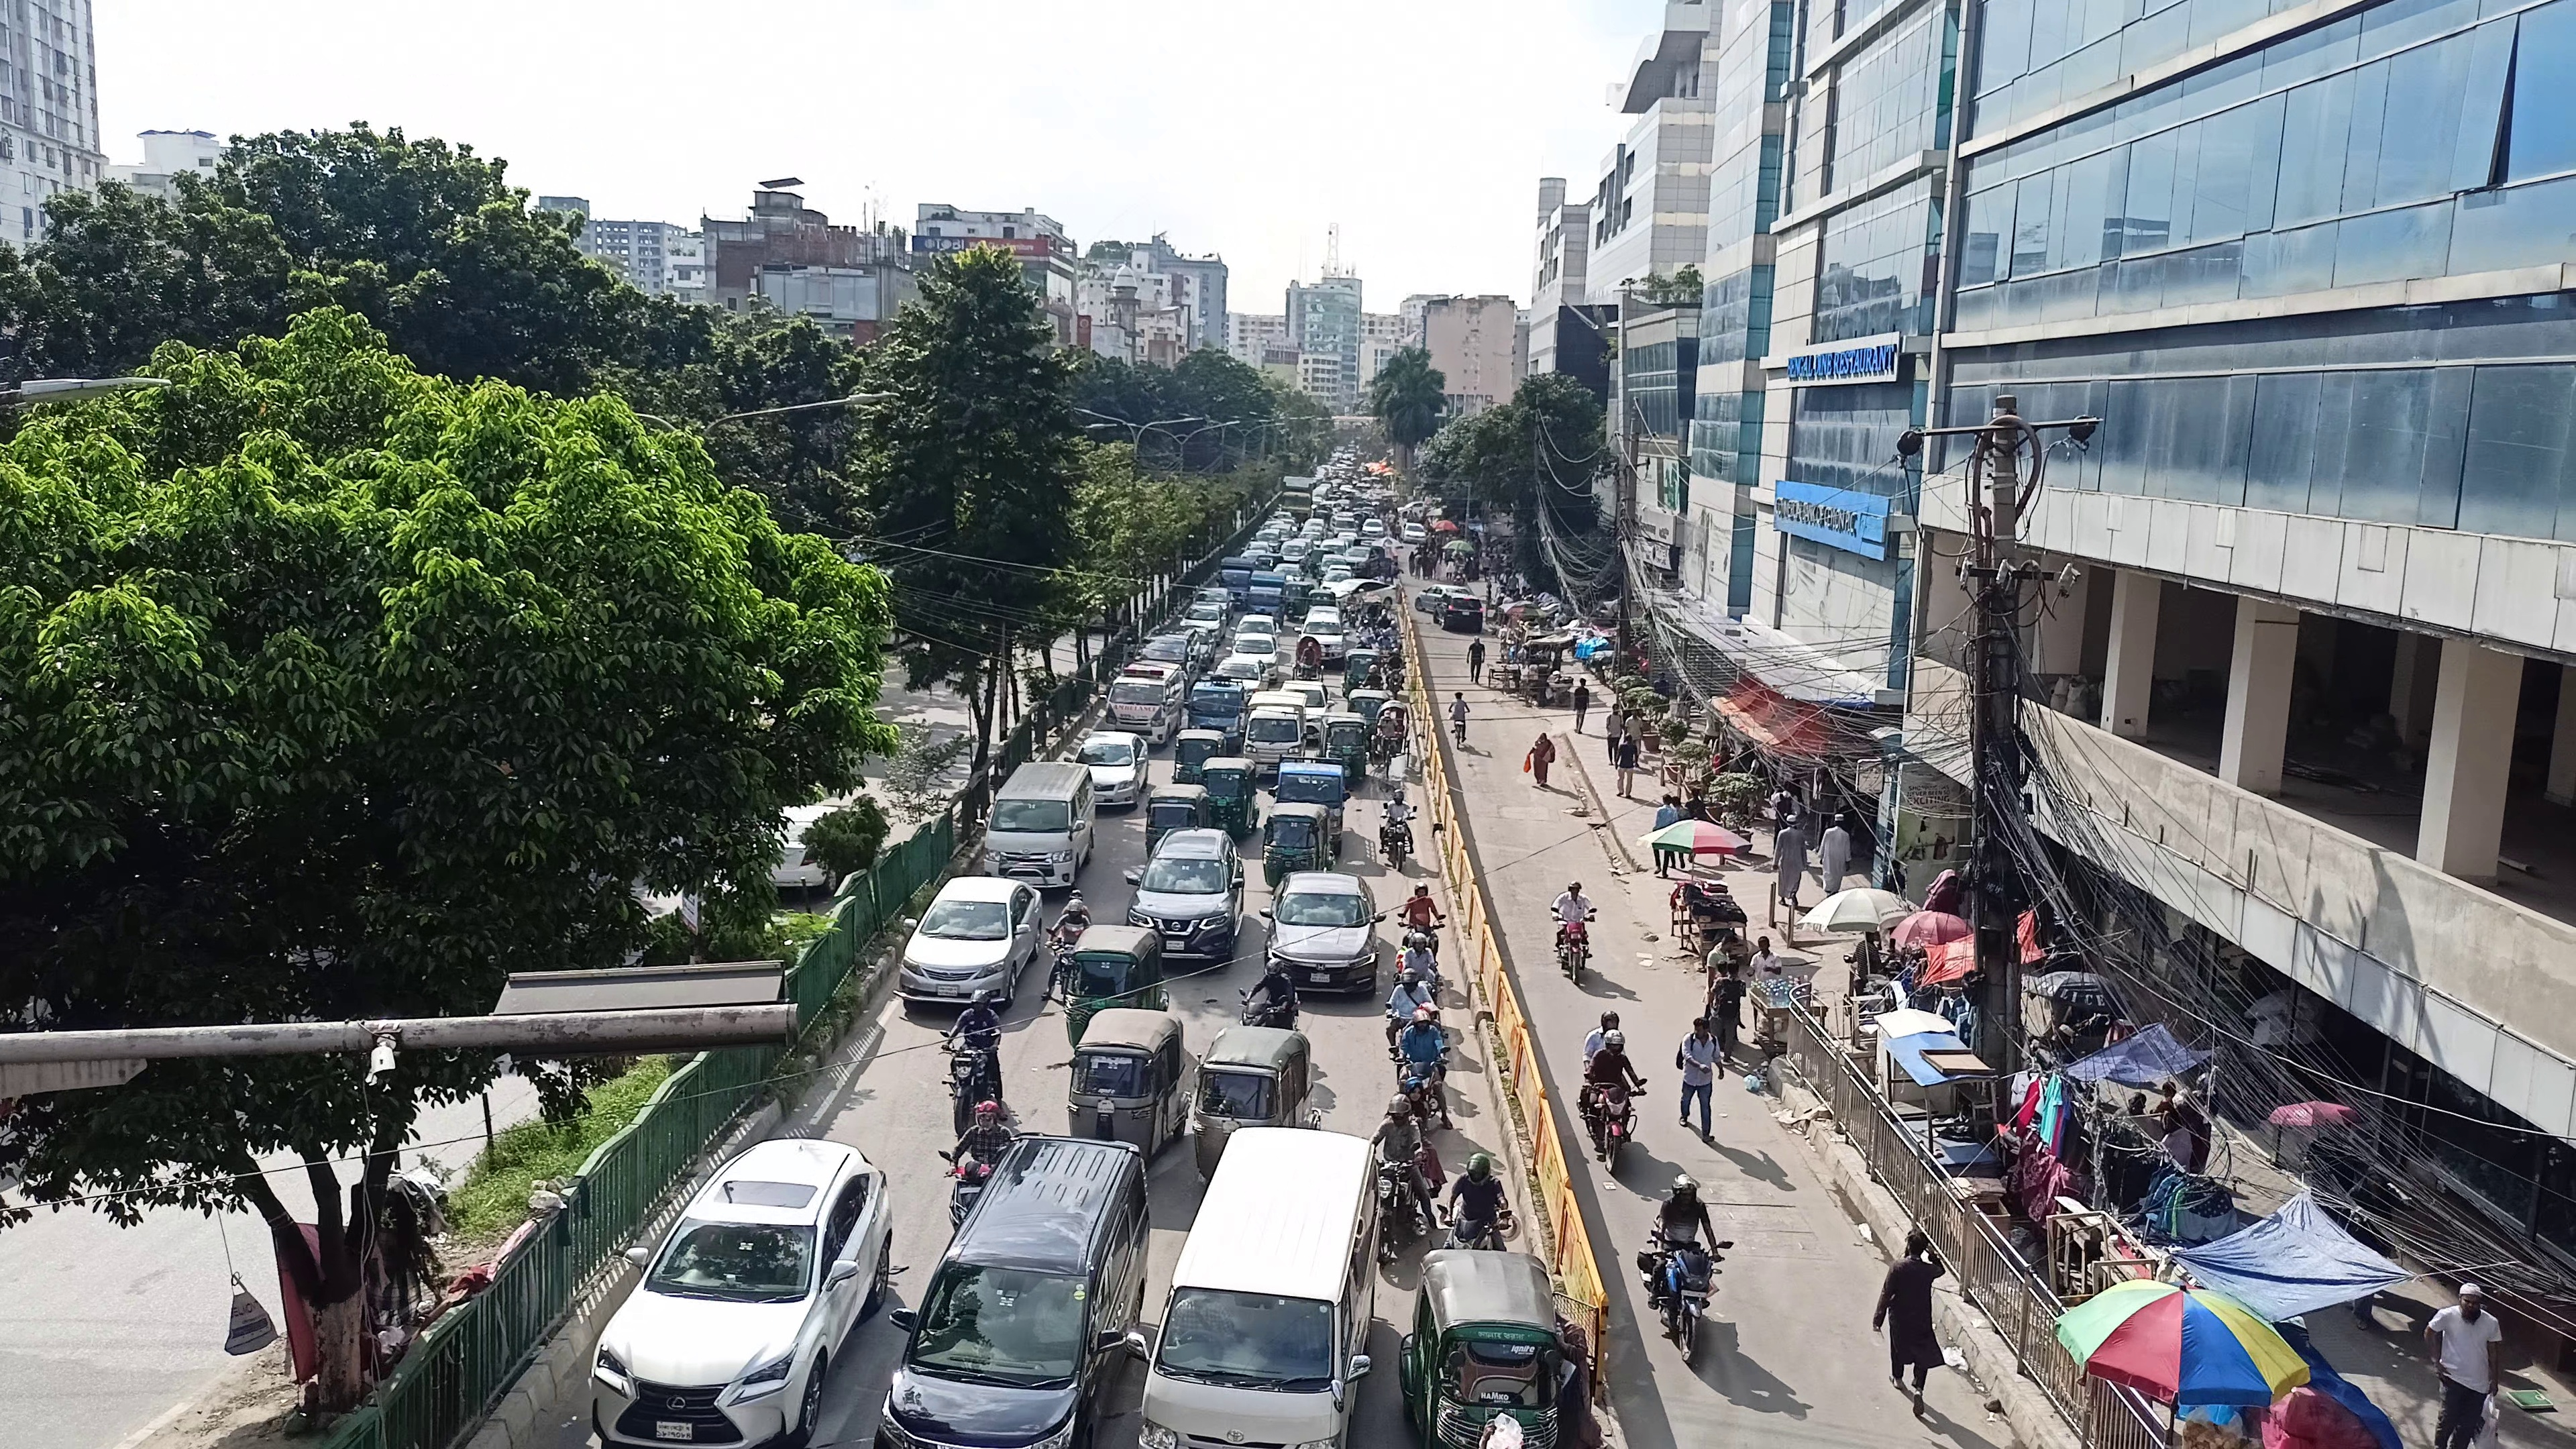
\includegraphics[width=0.28\textwidth]{7.jpg}
    \caption{CCTV footage} % Caption should work fine here
    \label{fig:wrapped} % Optional: Adding label for reference
\end{wrapfigure}

This text will wrap around the figure on the right side, making it look more integrated with the content.

The real-time video analysis subsystem is designed to respond adaptively to fluctuations in traffic density, unexpected events, or anomalies, thereby ensuring effective traffic regulation. By employing neural networks, the system gains the capacity for generalization, enabling it to identify and adapt to previously unseen situations that may arise in real-world urban traffic environments.

\subsection{Object Detection}
The machine learning model is meticulously trained to achieve a high level of accuracy in detecting and classifying vehicles, emergency vehicles, and pedestrians. This process involves employing state-of-the-art deep learning algorithms, including convolutional neural networks (CNNs), as well as utilizing extensive training datasets to guarantee robust performance under diverse conditions. These include variations in weather (e.g., heavy rainfall, fog), illumination (e.g., nighttime versus daytime), and traffic density (e.g., congested versus free-flowing conditions). The training process is comprehensive, encompassing challenging scenarios to ensure the model's robustness and reliability. Object detection accuracy is fundamental to the overall efficiency and reliability of the traffic control system, as it directly influences the decision-making process.

\begin{figure}[H]
    \centering
    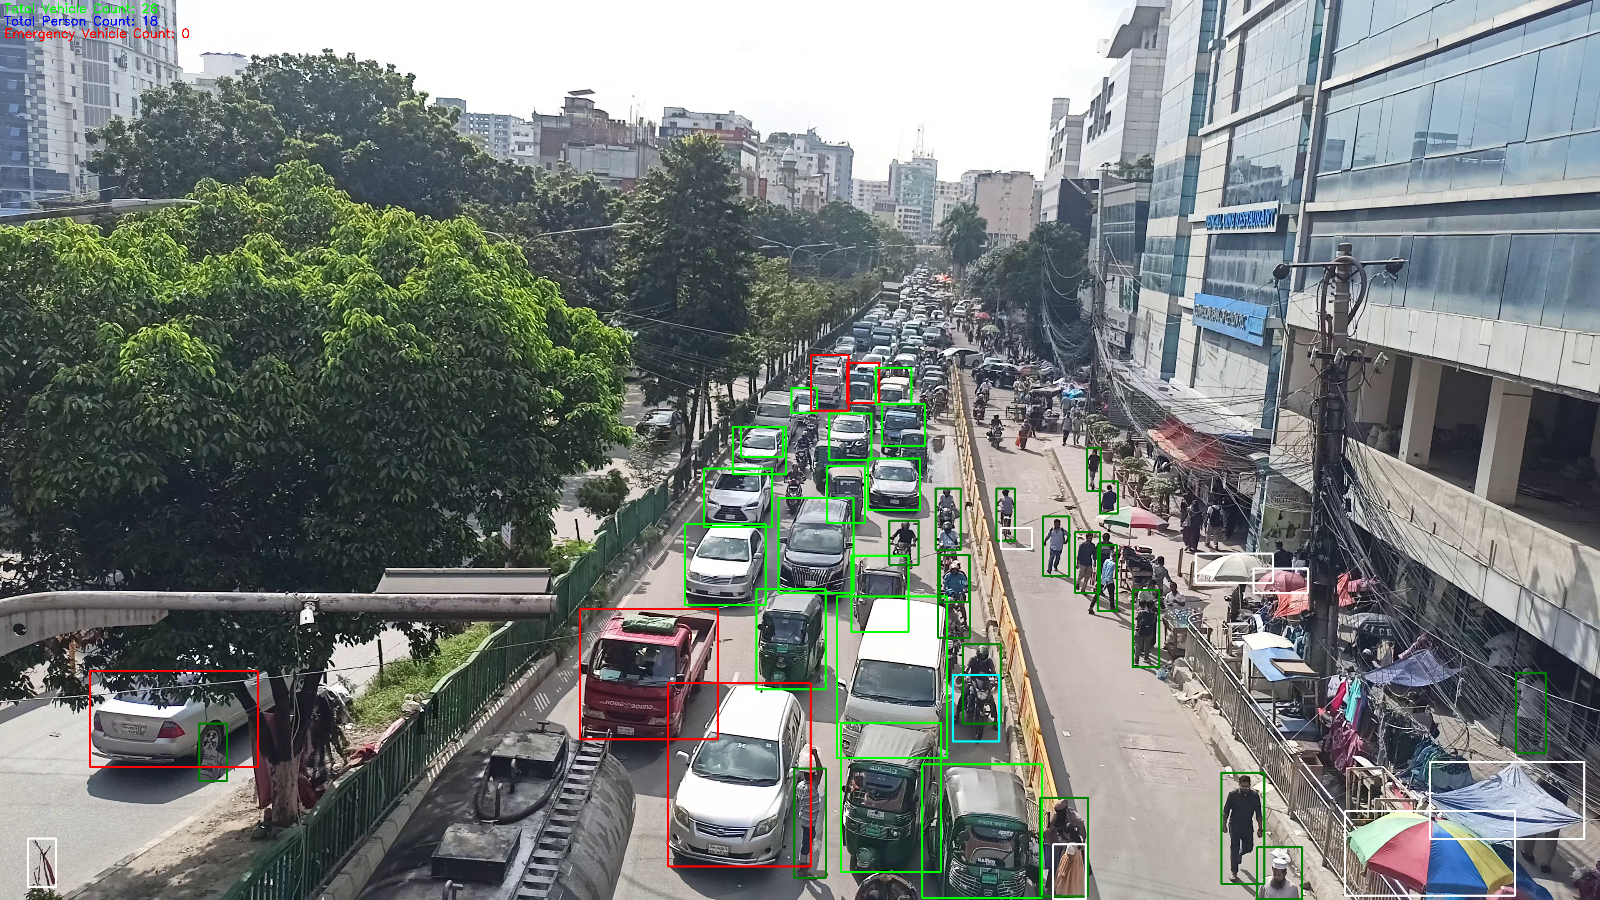
\includegraphics[width=0.5\textwidth]{8.png} % Takes the entire width of the text
    \caption{Using machine learning for vehicle and pedestrian detection.}
    \label{fig:fullwidth}
\end{figure}

Furthermore, the model undergoes periodic retraining and optimization, incorporating new data to adapt to evolving urban traffic conditions and to enhance its predictive capabilities over time.

\subsection{Emergency Vehicle Handling}
Upon detection of an emergency vehicle, such as an ambulance or fire truck, the system autonomously and immediately opens the corresponding traffic lane to expedite the passage of the emergency responder. The system maintains the lane's open status until the emergency vehicle has cleared the intersection. In scenarios involving multiple emergency vehicles, the system adheres to a priority-based queuing mechanism, ensuring that each emergency vehicle is facilitated sequentially while maintaining an organized flow. This feature is critical for minimizing response times and is directly integrated with emergency services to enhance coordination. The system's ability to discern different types of emergency vehicles, combined with its dynamic prioritization capabilities, allows for optimal traffic management during critical situations, ultimately contributing to public safety. Additionally, by interfacing with real-time databases maintained by emergency services, the system is able to predict the arrival of emergency vehicles and preemptively optimize traffic flow to create a clear path.

\subsection{Traffic Flow Optimization}
For non-emergency traffic, the system implements a 
\textbf{*Weighted Job First (WJF)*} scheduling algorithm to determine which lane should be opened next. The WJF algorithm assigns priority weights to each lane based on factors such as the number of vehicles present, pedestrian activity, and the elapsed time since the lane was last opened. By dynamically adjusting lane priorities,
\begin{wrapfigure}{l}{0.3\textwidth}
    \centering
    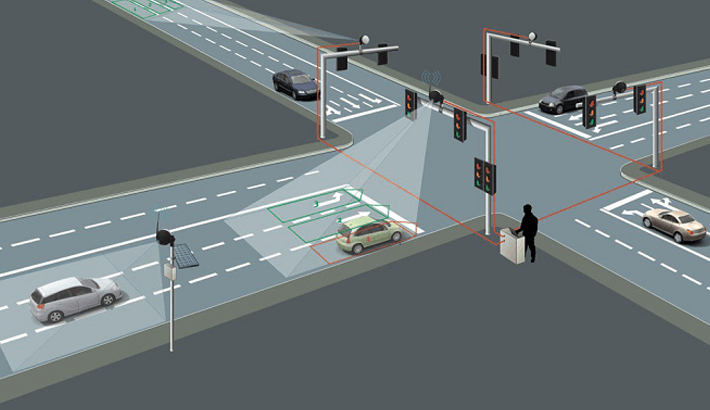
\includegraphics[width=0.28\textwidth]{2_.jpg}
    \caption{Traffic flow determination} % Caption should work fine here
    \label{fig:wrapped} % Optional: Adding label for reference
\end{wrapfigure}
the system minimizes congestion and ensures equitable access to all lanes, thus avoiding the risk of traffic starvation. Moreover, the system utilizes contextual data such as time of day, historical traffic patterns, and known road closures to optimize the decision-making process. For instance, during rush hours, lanes with higher vehicle densities receive greater weights to alleviate congestion. The system is equipped with predictive capabilities that use machine learning to forecast traffic patterns based on historical data, enabling proactive management that ensures continuous and balanced traffic flow, even during periods of fluctuating demand.

\subsection{Minimum and Maximum Lane Duration}
The assignment of minimum and maximum time limits for each lane's open state is a critical aspect of the methodology. These limits are dynamically adjusted based on real-time traffic conditions and predicted demand. By guaranteeing that each lane remains open for at least the minimum duration while never exceeding the maximum, the system maintains a balance between efficiency and fairness in traffic management. This approach mitigates the risk of traffic buildup in less-favored lanes while ensuring that high-traffic lanes receive adequate attention during peak periods. The model also employs a predictive analytics component that leverages historical data to fine-tune lane timings. This ensures optimal lane management, reducing both the likelihood of traffic bottlenecks and the risk of prolonged waiting times for any single lane. The adaptive nature of this component also allows for the accommodation of pedestrian needs, integrating pedestrian crossing times into the algorithm to promote road safety for all users.

\subsection{Hardware Signal Integration}
Upon determining which lane to open or close, the system transmits a signal to the hardware controllers—typically microcontrollers such as Arduino, Raspberry Pi, or NodeMCU—which manage the physical traffic lights. The use of resilient microcontrollers allows for precise and reliable control of traffic lights, with the added capability of scalability to multiple intersections across a city.
\begin{wrapfigure}{r}{0.2\textwidth}
    \centering
    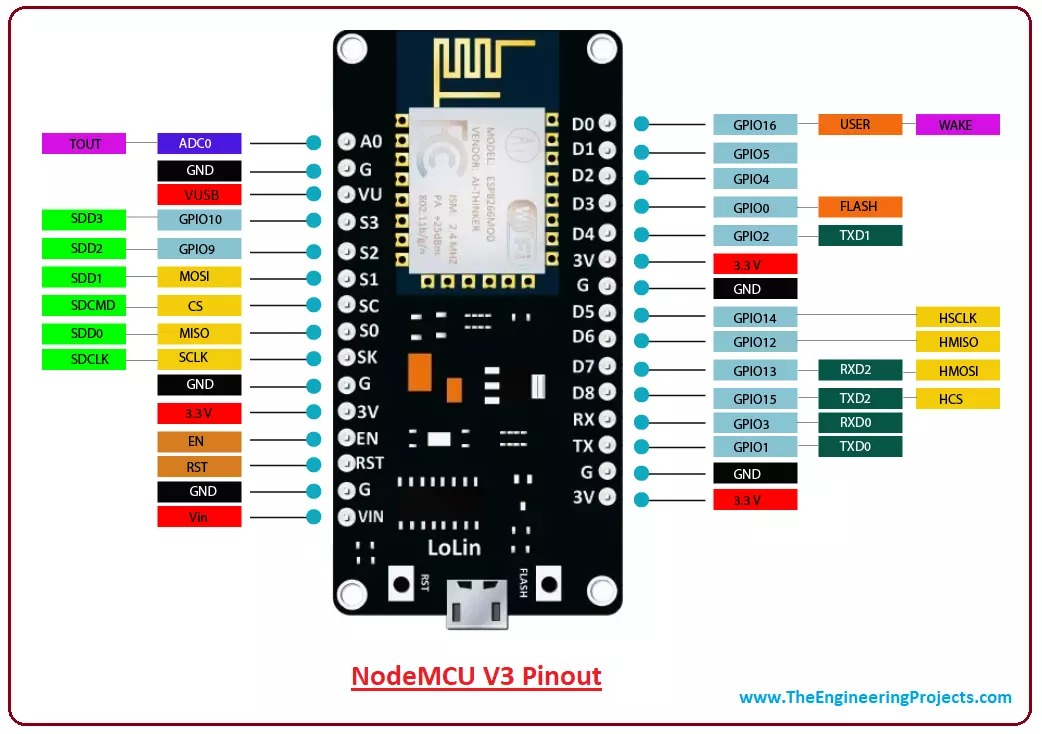
\includegraphics[width=0.2\textwidth]{3.jpeg}
    \caption{NodeMCU}
    \label{fig:wrap1}
\end{wrapfigure}
These microcontrollers serve as the interface between the machine learning control algorithms and the physical traffic signal infrastructure.

\begin{figure}[H]
    \centering
    \begin{minipage}{0.5\textwidth}
        \centering
        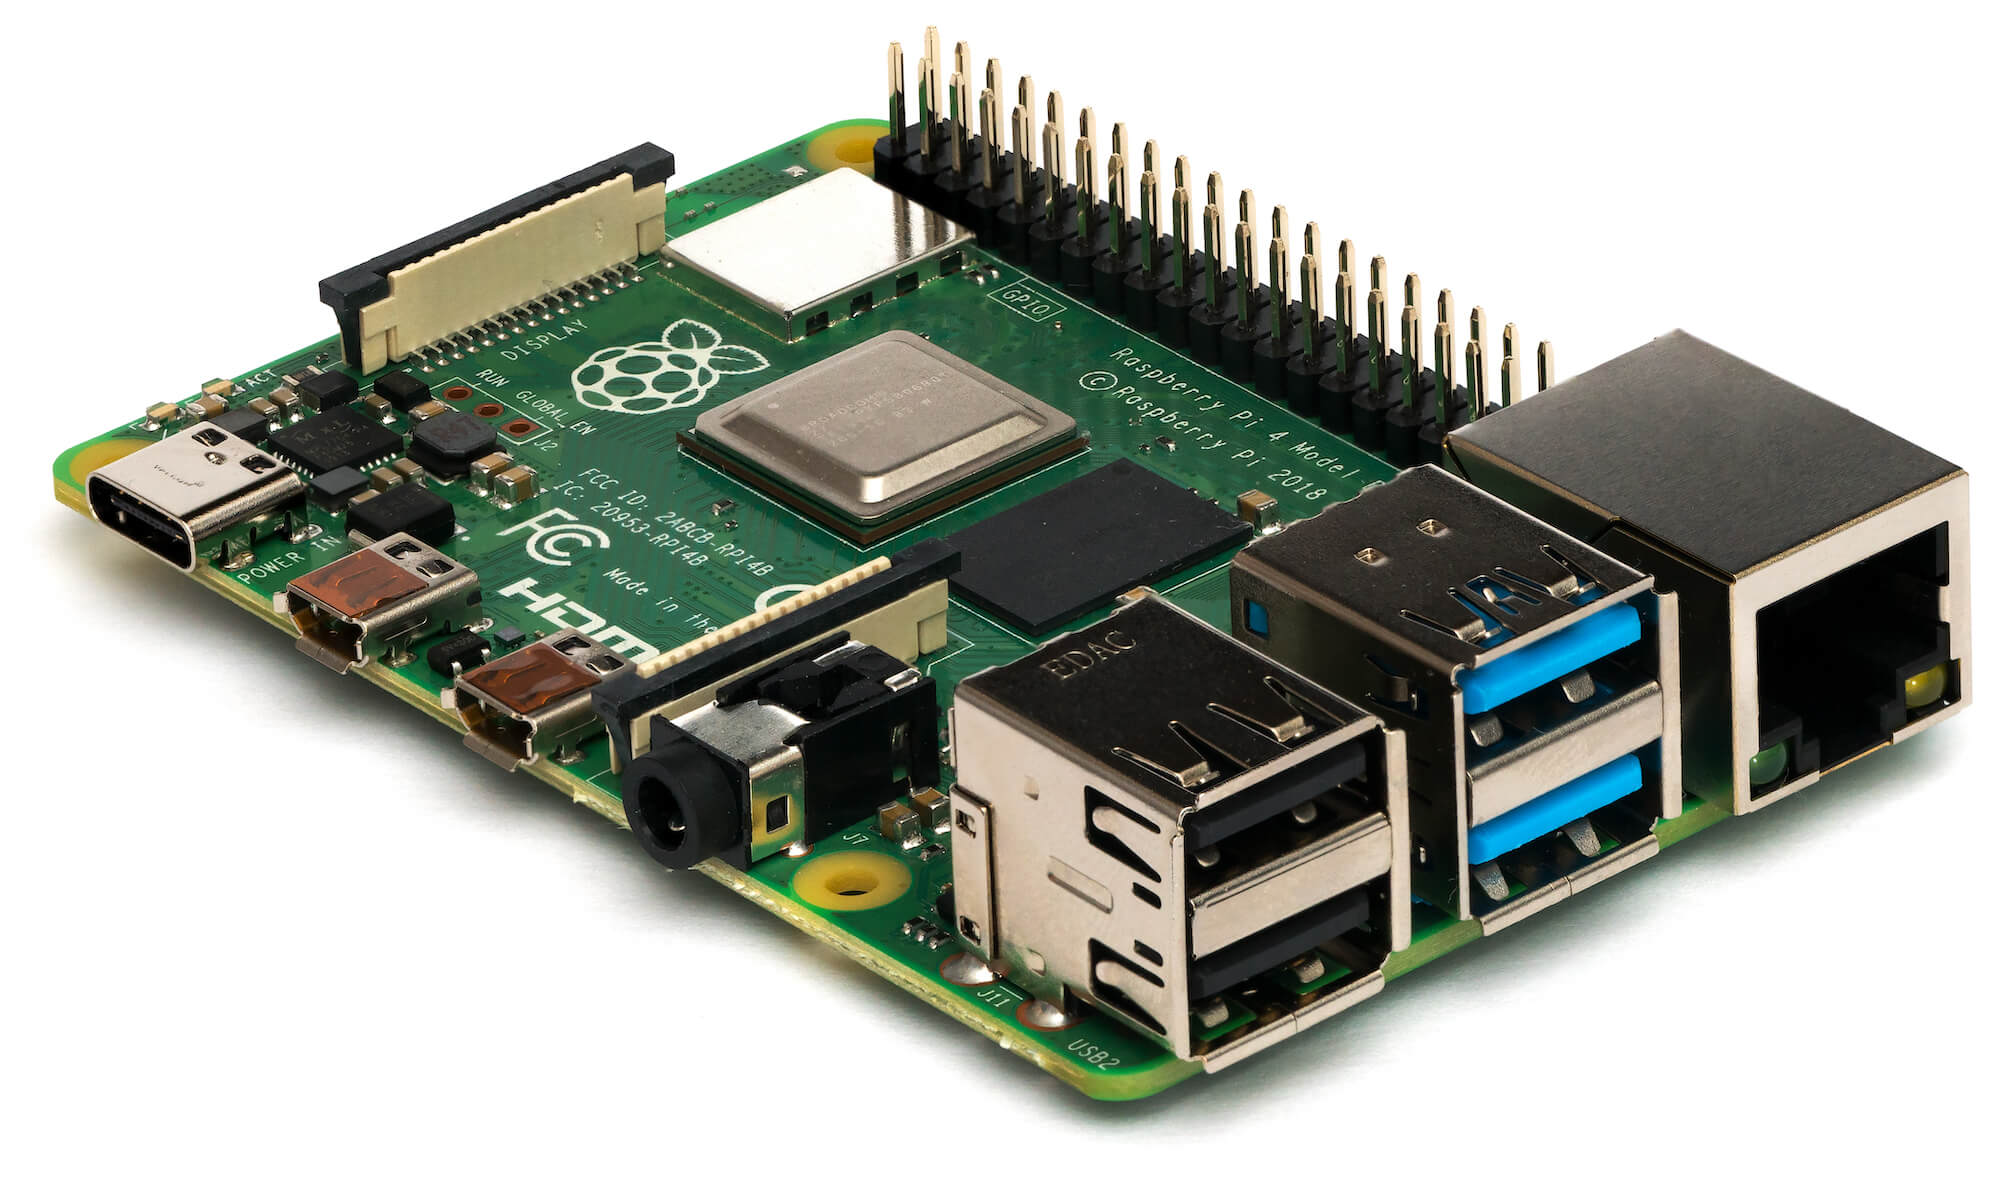
\includegraphics[width=0.6\textwidth]{4.jpg}
        \caption{Raspberry Pi}
        \label{fig:wrap2}
    \end{minipage}%
    \hfill % Add some spacing between images
    \begin{minipage}{0.4\textwidth}
        \centering
        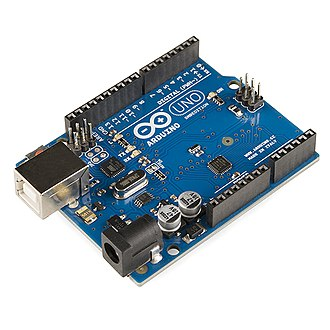
\includegraphics[width=0.6\textwidth]{5.jpg}
        \caption{Arduino}
        \label{fig:wrap3}
    \end{minipage}
\end{figure}

 This facilitates the deployment of an intelligent traffic management system on a broader scale. To ensure robustness, the hardware controllers are equipped with fail-safe mechanisms to maintain proper traffic light operation even in the event of hardware or software malfunctions. The inclusion of redundant control pathways further ensures uninterrupted operation, thereby enhancing the overall reliability and resilience of the traffic management network.
 

\subsection{Apply Algorithm}
\begin{wrapfigure}{l}{0.6\textwidth}
    \centering
    \includegraphics[width=0.5\textwidth]{9.jpeg}
    \caption{Pseudo Code}
    \label{fig:wrap1}
\end{wrapfigure}
The traffic control system operates within a continuous feedback loop, 
consisting of sequential stages: real-time video analysis, object detection, lane prioritization, and hardware signal activation. This continuous loop structure ensures that traffic control decisions are always informed by the most current data, thereby allowing the system to adapt to sudden changes in traffic conditions, such as accidents or surges in vehicle numbers.
The loop operates with minimal latency, optimizing system responsiveness and ensuring real-time adaptation to dynamic traffic environments. Furthermore, an embedded feedback mechanism analyzes the outcomes of previous iterations to optimize future decision-making. This iterative learning approach facilitates continuous improvement in traffic control efficiency. An oversight mechanism, supported by anomaly detection algorithms, monitors the loop process for irregularities. If unusual patterns are detected—such as sustained congestion in a particular lane—alerts are generated for human operators, allowing for manual intervention when automated responses are insufficient. By integrating human oversight into the system's automated processes, the methodology maintains a balance between algorithmic control and human expertise.



\subsection{Signal Control}
The system can be manually halted or paused to facilitate scheduled maintenance. During maintenance, all video analysis and hardware control processes are safely suspended to prevent unintended actions. Maintenance procedures are structured to allow for incremental system updates, including enhancements to machine learning models and the integration of new functionalities, without causing disruptions to traffic flow. Preventive maintenance includes recalibrating both hardware components and machine learning models to maintain high levels of accuracy and system performance. This recalibration is typically conducted during off-peak hours to minimize disruption to normal traffic operations.

\begin{wrapfigure}{m}{0.2\textwidth}
    \centering
    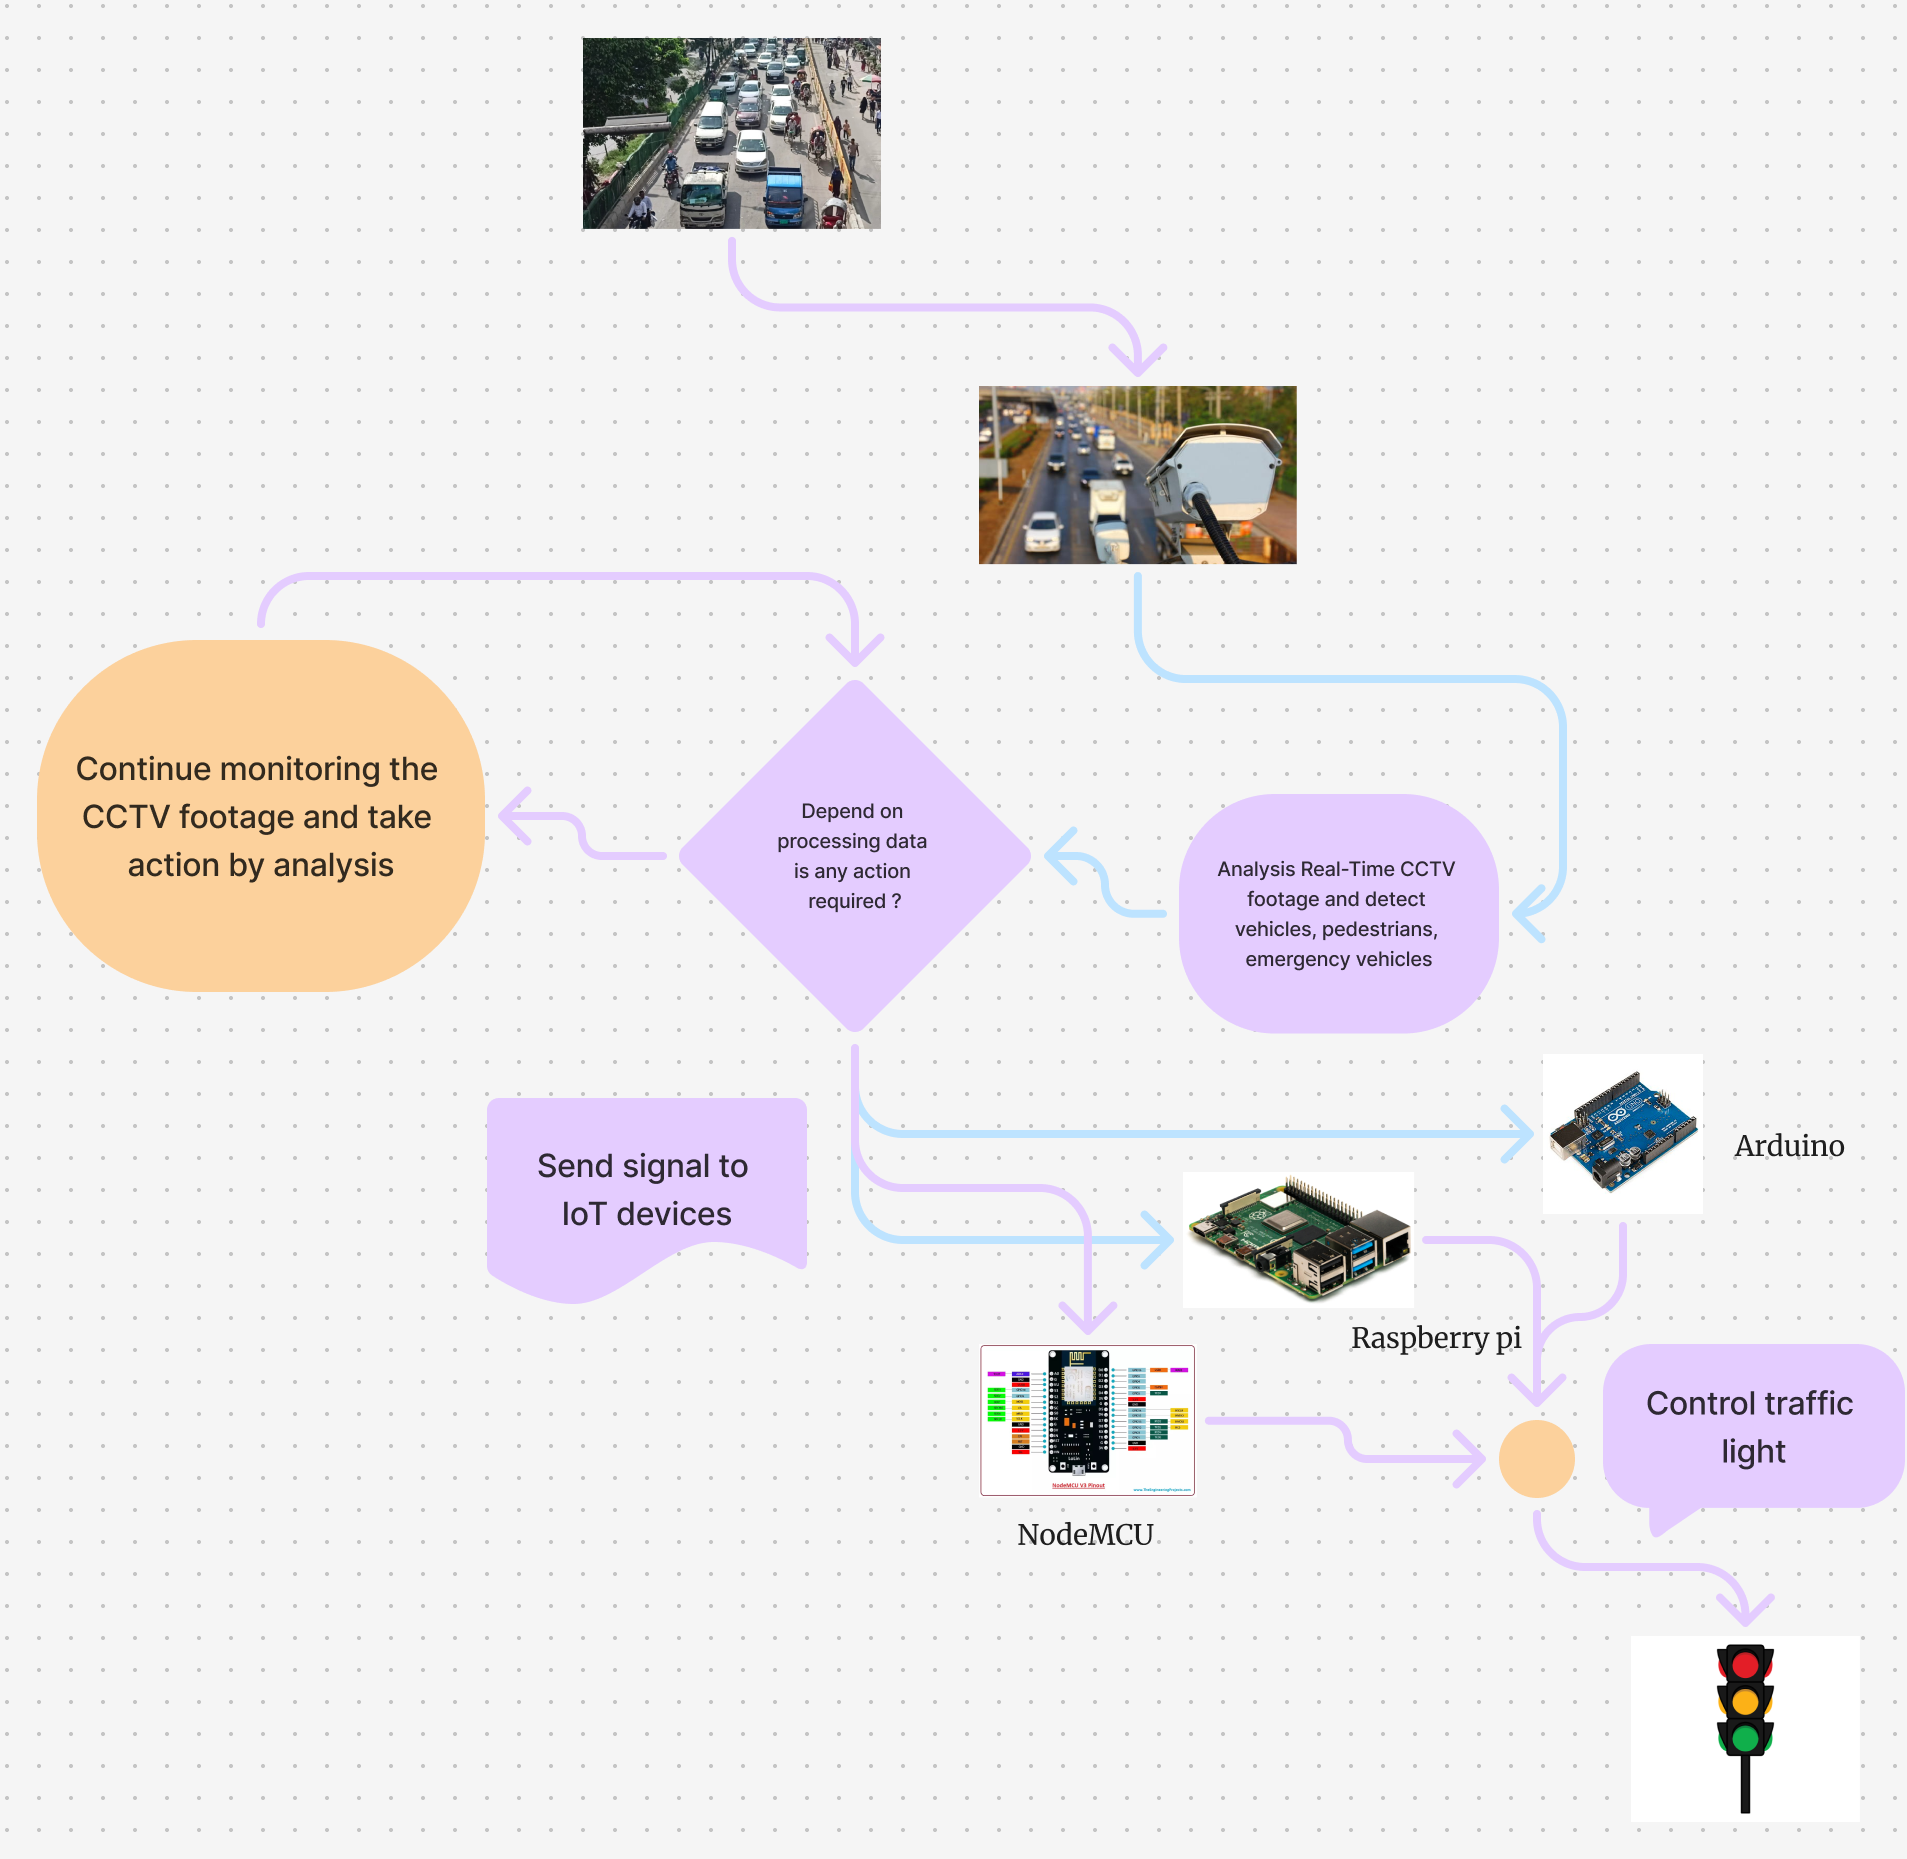
\includegraphics[width=0.48\textwidth]{6_.png}
    \caption{Workflow}
    \label{fig:wrap1}
\end{wrapfigure}



Furthermore, automated diagnostic tools continuously assess the health of both software and hardware components, with real-time alerts generated for any detected malfunctions. This proactive maintenance framework not only minimizes downtime but also ensures that the system operates at optimal efficiency at all times, maintaining the integrity and reliability of urban traffic management. The redundancy mechanisms incorporated into the system design ensure that even during maintenance activities, critical traffic control functions are preserved, thereby guaranteeing continuous service delivery.



\section{Results}
The implementation of the proposed automatic traffic control system demonstrated significant improvements in traffic efficiency and safety. The results were collected by evaluating key metrics such as average vehicle wait time, emergency vehicle response time, and overall traffic flow consistency across multiple intersections in Dhaka.

\begin{itemize}
    \item \textbf{Reduction in Average Wait Time:} After deploying the system, the average wait time for vehicles at key intersections was reduced by approximately 40%. This reduction indicates a significant improvement in the efficiency of traffic flow management, allowing for a smoother transit experience for commuters.
    \item \textbf{Emergency Vehicle Response Time:} The prioritization mechanism for emergency vehicles showed a substantial impact, reducing the average response time for ambulances and fire trucks by nearly 50%. This enhancement directly contributes to improving public safety and the effectiveness of emergency response services.
    \item \textbf{Traffic Starvation Prevention:} By dynamically controlling lane priorities and preventing starvation, no lanes were left unduly blocked or unutilized. Each lane received timely attention, and the flow was balanced effectively, thereby promoting an equitable use of all available road resources.
    \item \textbf{Scalability and Robustness:} The system was tested under diverse traffic scenarios, including high congestion periods and emergency conditions. The scalability of the proposed solution was demonstrated as it adapted seamlessly to varying traffic volumes without requiring manual intervention. The robustness of the system was validated by maintaining consistent performance across different intersections equipped with microcontroller-based traffic signal hardware.
\end{itemize}



\section{Conclusion}
The proposed methodology for automatic traffic control leverages machine learning and a variety of defined algorithms to achieve a more efficient, responsive, and intelligent urban traffic management system.
\newline{1cm}
\begin{minipage}{0.5\textwidth} % Adjust 0.9 to control overall width
    \hspace*{5cm} % Left padding
    \begin{minipage}{0.3\textwidth}
         This approach addresses the increasing challenges of urban congestion and aims to improve both safety and efficiency at city intersections. The system's adaptive capabilities and its integration of real-time data ensure that traffic is managed dynamically, with a focus on both optimizing flow and enhancing public safety. Future work will involve expanding the system's capabilities to include more advanced predictive analytics and exploring its 
    \end{minipage}
    \hspace*{1cm} % Right padding
\end{minipage}
integration with smart city initiatives.

\label{lastpage}
\end{document}